\chapter{Design}\label{design}

Significant design work has been performed for this system at both the architectural level and user interface. Interface design is discussed in section \ref{screen_design}. 

I have chosen to implement a client server model for the system architecture, as this offers a strong separation into multiple loosely coupled modules. Given a client server architecture, and a desire for centralised data storage between multiple users a browser based approach was chosen. Using existing browsers leverages significant work done on secure network communications between client and server, as well as significant effort in sand-boxing (isolating from the rest of the computer) in-browser applications. This saves significant time and effort on implementing communication protocols and security. 

As there are relatively few programming languages available for use within the browser this significantly simplified the choice of languages and tool sets. See section \ref{langs}.

\begin{figure}[tbh]
\fbox{\parbox[b]{.99\linewidth}{
\vskip 0.5cm
\centering 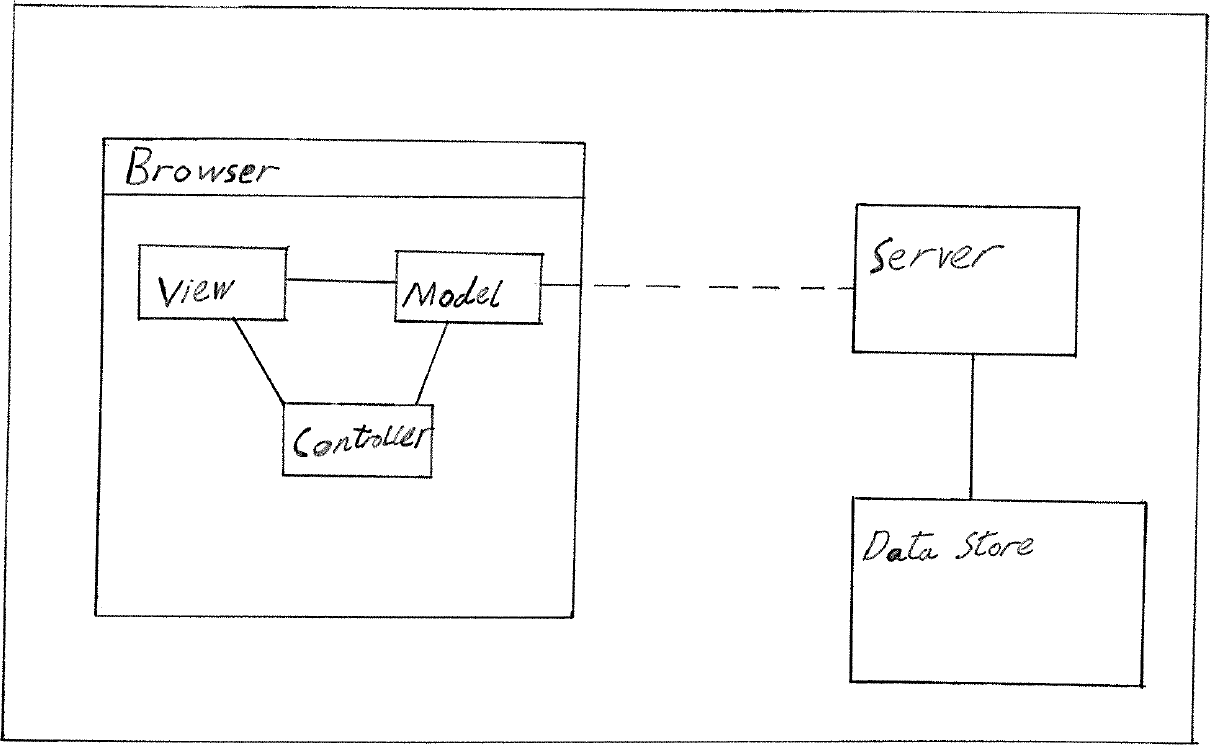
\includegraphics[scale=0.3]{blocks.png}
\vskip 0.5cm}}
\caption{\protect\label{spiral_plan}Block diagram showing proposed architecture of system. Note complete separation between server and browser. These may reside on separate machines.}
\end{figure}

Inside the browser there are three major components from an object oriented perspective. The view contains what is actually displayed on screen, this is implemented in HTML with SVG (Scalable Vector Graphics) for graphical components. The model stores the data and handles requests to the server as necessary. The controller is responsible for implementing user interaction with the system.

Communication between the client and server is handled through standardised protocols. The set of requests permissible is still to be defined. The server software is responsible for serving data to the client, performing data aggregation, and limited data mining. In order to provide data, the server communicates with the data-store. This communication is likely to take place through SQL to a database, though a modular design could permit creation of other storage interface modules.

Data aggregation is performed server side for two reasons. In larger networks, or over longer time periods, many megabytes of logs can be created, while text is highly compressible this still creates significant network overhead to transfer. Further, there are unanswered questions about how well the client will perform with potentially millions of events to manipulate. Slow data transfers or interaction due to processing time would be a significant usability hurdle. Performing data aggregation on the server bypasses both of these limitations. 

\subsection{User interface design}\label{screen_design} 
  
I have chosen to adopt a time based approach for the visualisation elements, as access attempt logs have a very strong time component. Some forms of unusual behaviour are evidenced only by unusual times for access attempts, or unusual durations of access for example. Most existing visualisations do not give much emphasis to the time relation between access attempts, preferring to focus on the links between source and destination addresses.

Two major approaches have been considered for displaying log entries.
Spiral view is an approach for displaying time series data mapped to a spiral, see figure \ref{spiral} where a straight line drawn from the outer edge to the center shows the same time at each level of the spiral \cite{bertini2007spiralview, chin2009visual}
These systems appear to be highly effective at displaying time series data in a fashion that supports easy detection of repeated patterns. 

\begin{figure}[tbh]
\fbox{\parbox[b]{.99\linewidth}{
\vskip 0.5cm
\centering 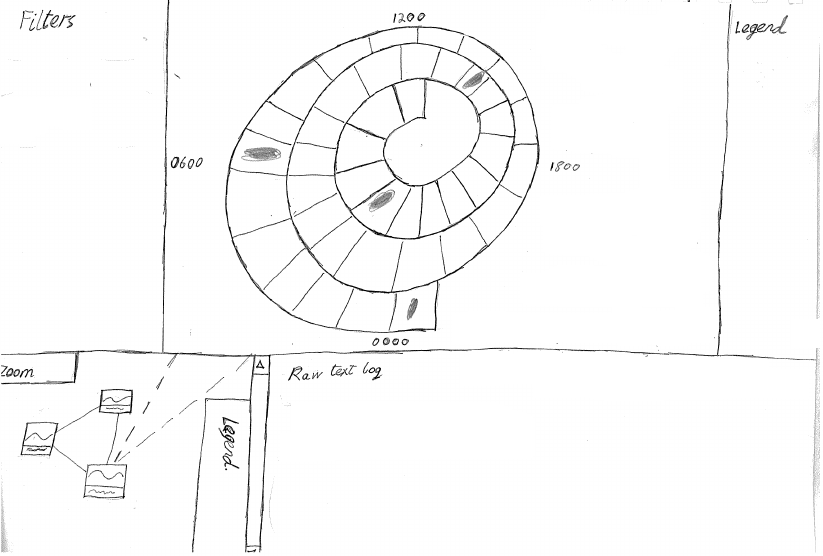
\includegraphics[scale=0.75]{spiral_plan.png}
\vskip 0.5cm}}
\caption{\protect\label{spiral_plan}Drawing showing proposed layout using spiralview for main focus. Black shading shows selection of an event with highlighting of related events.}
\end{figure}
 
However serious flaws in the results(\cite{chin2009visual}) of usability tests presented have lead to the rejection of this method. The error in question shows a table of results that directly contradict claims made in the text about how well spiralview supports the detection of patterns. The claims contradicted in the work are those directly bearing on the uses I had intended for the spiral layout. As this is a 300 hour project, I will not be attempting to repeat their work to clarify their findings. I attempted to contact the authors of the paper, and have as yet received no response.

This contradiction has lead to using a simpler and better understood layout for time series data. 

\begin{figure}[tbh]
\fbox{\parbox[b]{.99\linewidth}{
\vskip 0.5cm
\centering 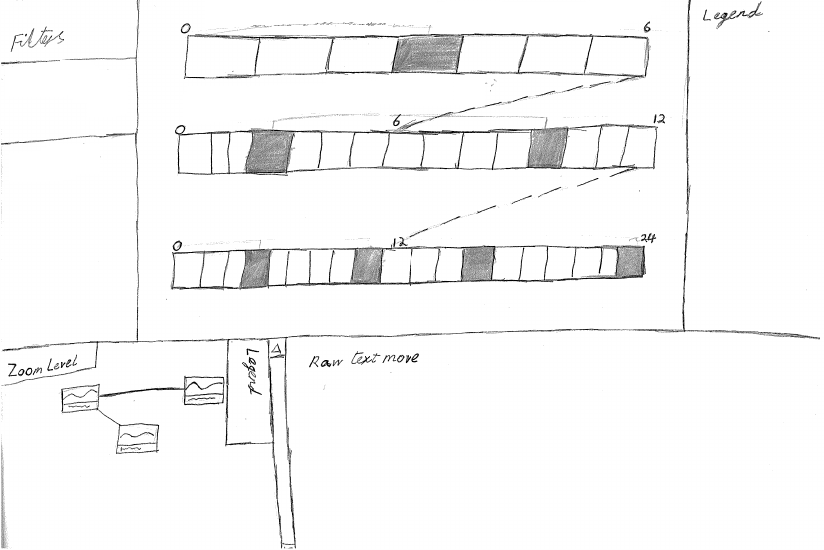
\includegraphics[scale=0.75]{lines.png}
\vskip 0.5cm}}
\caption{\protect\label{lines}Drawing showing proposed layout using multiple time lines for main focus. Black shading shows selection of an event, with highlighting related events.}
\end{figure}

Using block representation of data arranged linearly along a time axis.
Initial designs called for using a stacked representation where each layer represented twice the time of the previous layer.
This is proposed to show patterns as an element that repeats a growing number of times in each layer.
Tufte's work on small multiples \cite{tufte1983visual} suggests keeping each level of the stack to represent the same amount of time, with differing start and end points. Ie: if the range is 6 hours, the top bar starts at 0600, and runs to 1200, the one below it from 0000 to 0600..  and so on. This would show patterns repeating with a period less than the time range by showing in multiple bars. See Figure \ref{lines}.

I have been forced to consider data hiding techniques, as networks can become extremely busy, producing sufficient activity to overwhelm the user's ability to absorb information and detect meaningful patterns in the clutter. As I have chosen a time series based approach to displaying the data, I have chosen to use time binning to aggregate entities. This approach is extremely simple, with all entries in a short time period displayed as a single entity, with icons indicating some simple features of the hidden data. Such features include superuser accesses, abnormal numbers of failed access attempts, abnormally large numbers of access attempts, abnormal login locations for a user, abnormal login times for a user. Each time bin can be zoomed in on, allowing the user to see greater detail within the bin. For extremely busy systems and longer time periods there may be multiple levels of binning in play to aggregate sufficiently. This scheme reduces the visual complexity, while allowing easy access to detailed information about each incident. 

These last are the most complicated flags, as they require creating a profile of each user's access times over repeated access attempts. This complexity can produce false positives while the system is learning a new user's habits. and may be tripped up by a legitimate change in user habits.

\subsection{Parser}
why do clustering here?

\subsection{Server}
why two layer architecture - ease of shifting datastore, changes there are isolated from server and thus web app, may find more appropriate datastore for semistructured log data in future. - why not three?
Only one servlet has any data processing outside of database, so third layer usually unneccessary, and overkill in the one case where some processing needed.

\subsection{Database}
RDBMS acceptable fit for log data, though relatively unstructured data leads to less than ideal schema. why use RDBMS? lack of knowlege of alternatives, already available through university. handles concurrent accesses well.. many alternates leave concurrency issues to client code.


\section{Requirements}
discuss here some thoughts as to what requirements were met, and which were abandoned for time limitations.
requirements for log parsing limited to SSHD logs, not limited to one ssh demon.
network context dropped.



